% ==============================================================================
% FYDP-I Defense Slides
% "Solving the Lorenz ODE System Using Optimal ANN Architectures"
% United International University - Department of CSE
% Theme matched to the institutional reference deck (teal / mint).
% Built from scientific-slides defense template, reusing paper figures.
% Compile: pdflatex defense_slides.tex  (run twice for slide totals)
% ==============================================================================
\documentclass[aspectratio=169,11pt]{beamer}

\usepackage[utf8]{inputenc}
\usepackage[T1]{fontenc}
\usepackage{lmodern}
\usepackage{graphicx}
\usepackage{amsmath,amssymb}
\usepackage{booktabs}
\usepackage{array}
\usepackage{colortbl}
\usepackage[most]{tcolorbox}
\graphicspath{{./figures/}}

% ---------------------------------------------------------------- colour palette
\definecolor{tealDark}{RGB}{62,124,116}   % section bars / title bar
\definecolor{tealMid}{RGB}{143,196,189}   % card frames
\definecolor{tealSoft}{RGB}{206,231,228}  % card fill
\definecolor{tealPale}{RGB}{243,250,249}  % slide background
\definecolor{ink}{RGB}{32,46,44}          % body text
\definecolor{accent}{RGB}{223,150,64}     % sparing orange accent

% ---------------------------------------------------------------- base theme
\usetheme{default}
\usefonttheme{professionalfonts}
\setbeamertemplate{navigation symbols}{}
\setbeamercolor{normal text}{fg=ink}
\setbeamercolor{background canvas}{bg=tealPale}
\setbeamercolor{structure}{fg=tealDark}
\setbeamercolor{itemize item}{fg=tealDark}
\setbeamercolor{itemize subitem}{fg=tealMid}
\setbeamerfont{frametitle}{series=\bfseries,size=\Large}
\setbeamerfont{title}{series=\bfseries}

% teal title bar
\setbeamercolor{frametitle}{bg=tealDark,fg=white}
\setbeamertemplate{frametitle}{%
  \nointerlineskip%
  \begin{beamercolorbox}[wd=\paperwidth,ht=2.6ex,dp=1.2ex,leftskip=0.6cm,rightskip=0.6cm]{frametitle}%
    \usebeamerfont{frametitle}\insertframetitle%
  \end{beamercolorbox}%
}

% footline: short title (left) | author (centre) | frame number (right)
\setbeamercolor{footline}{fg=white,bg=tealDark}
\setbeamertemplate{footline}{%
  \leavevmode%
  \hbox{%
  \begin{beamercolorbox}[wd=.40\paperwidth,ht=2.4ex,dp=1ex,leftskip=.4cm]{footline}%
    \footnotesize Lorenz-1960 $\times$ ANN%
  \end{beamercolorbox}%
  \begin{beamercolorbox}[wd=.40\paperwidth,ht=2.4ex,dp=1ex,center]{footline}%
    \footnotesize FYDP-I Defense \textbullet\ UIU CSE%
  \end{beamercolorbox}%
  \begin{beamercolorbox}[wd=.20\paperwidth,ht=2.4ex,dp=1ex,rightskip=.4cm]{footline}%
    \hfill\footnotesize\insertframenumber\,/\,\inserttotalframenumber%
  \end{beamercolorbox}}%
  \vskip0pt%
}

% ---------------------------------------------------------------- card helpers
% titled card (mimics the reference deck's rounded teal cards)
\newtcolorbox{card}[1]{%
  enhanced, sharp corners=all, arc=3mm, boxrule=0pt, frame hidden,
  colback=tealSoft, coltext=ink,
  colbacktitle=tealMid, coltitle=ink, fonttitle=\bfseries\centering,
  title=#1, halign title=center,
  left=3mm,right=3mm,top=2mm,bottom=2mm, before skip=2pt, after skip=2pt}
% plain fill card (no title)
\newtcolorbox{plaincard}{%
  enhanced, sharp corners=all, arc=3mm, boxrule=0pt, frame hidden,
  colback=tealSoft, coltext=ink, left=3mm,right=3mm,top=2mm,bottom=2mm}

\newcommand{\stat}[2]{{\color{tealDark}\textbf{#1}}\\[-1pt]{\footnotesize #2}}

\begin{document}

% =============================================================== 1. TITLE
{\setbeamertemplate{footline}{}
\begin{frame}[plain]
  \centering
  \vspace{0.3cm}
  
\includegraphics[height=1.7cm]{uiu.png}\\[0.3cm]
  {\color{tealDark}\rule{0.86\textwidth}{1.2pt}}\\[0.25cm]
  {\Large\bfseries Solving the Lorenz ODE System\\[2pt] Using Optimal ANN Architectures}\\[0.2cm]
  {\color{tealDark}\rule{0.86\textwidth}{1.2pt}}\\[0.35cm]
  {\footnotesize Final Year Design Project I \textbullet\ Department of CSE, United International University}\\[0.45cm]
  \begin{columns}[t]
    \column{0.62\textwidth}
      \centering\footnotesize
      \textbf{Team Members}\\[2pt]
      Ikramul Hasan Moral (0112230489)\\
      Md.\ Abu Bakar (0112230200)\\
      Samiur Rahman Omlan (0112230195)\\
      Fariha Islam (0112230431)\\
      Md.\ Touhidul Islam (0112230435)
    \column{0.38\textwidth}
      \centering\footnotesize
      \textbf{Supervisor}\\[2pt]
      Dr.\ Muhammad Nomani Kabir\\
      Professor, Department of CSE\\[8pt]
      \textbf{Date}\\[2pt]
      \today
  \end{columns}
\end{frame}
}

% =============================================================== 2. OUTLINE
\begin{frame}{Outline}
  \begin{columns}[T]
    \column{0.5\textwidth}
      \begin{enumerate}
        \item Problem \& Motivation
        \item Objectives
        \item Background: Lorenz-1960 \& ANNs
        \item Literature Review
        \item Research Gap \& Questions
      \end{enumerate}
    \column{0.5\textwidth}
      \begin{enumerate}
        \setcounter{enumi}{5}
        \item Methodology
        \item Progress: Validated Baseline
        \item Project Plan \& FYDP-II
        \item Conclusion
      \end{enumerate}
  \end{columns}
  \vspace{0.4cm}
  \begin{plaincard}
    \centering FYDP-I deliverable: a \textbf{validated numerical baseline} and a \textbf{controlled experimental design}
    for the ANN architecture search carried out in FYDP-II.
  \end{plaincard}
\end{frame}

% =============================================================== 3. PROBLEM
\begin{frame}{Problem \& Motivation}
  \begin{columns}[t]
    \column{0.33\textwidth}
      \begin{card}{No closed form}
        \footnotesize Coupled nonlinear ODEs like Lorenz-1960 rarely admit a closed-form solution.
      \end{card}
    \column{0.33\textwidth}
      \begin{card}{Classical solvers are costly}
        \footnotesize RK4 is accurate but mesh-dependent and must \emph{re-solve} step-by-step for every query.
      \end{card}
    \column{0.33\textwidth}
      \begin{card}{Neural methods lean on physics}
        \footnotesize Most ODE networks add physics-informed losses or operator learning.
      \end{card}
  \end{columns}
  \vspace{0.35cm}
  \begin{plaincard}
    \centering\textbf{Central question:} can a \textcolor{tealDark}{\bfseries plain feedforward ANN} ---
    trained only on numerical reference data, with no physics in the loss --- learn the Lorenz-1960 solution,
    and \emph{which architecture does it best}?
  \end{plaincard}
\end{frame}

% =============================================================== 4. OBJECTIVES
\begin{frame}{Objectives}
  \begin{columns}[t]
    \column{0.5\textwidth}
      \begin{card}{Build a trusted reference}
        \footnotesize
        \begin{itemize}
          \item Solve Lorenz-1960 with RK4 \emph{and} SciPy
          \item Cross-validate the two solvers
          \item Use the verified trajectory as ground truth
        \end{itemize}
      \end{card}
      \vspace{0.2cm}
      \begin{card}{Search the architecture space}
        \footnotesize
        \begin{itemize}
          \item Vary depth, width, activation
          \item Keep the network plain (no physics aids)
        \end{itemize}
      \end{card}
    \column{0.5\textwidth}
      \begin{card}{Evaluate accuracy vs.\ cost}
        \footnotesize
        \begin{itemize}
          \item MSE, MAE, max error
          \item Training and inference time
          \item Convergence stability
        \end{itemize}
      \end{card}
      \vspace{0.2cm}
      \begin{card}{Benchmark against literature}
        \footnotesize
        \begin{itemize}
          \item Compare with PINN / DeepONet results
          \item Position plain ANN against physics-informed methods
        \end{itemize}
      \end{card}
  \end{columns}
\end{frame}

% =============================================================== 5. BACKGROUND: SYSTEM
\begin{frame}{Background: The Lorenz-1960 System}
  \begin{columns}[c]
    \column{0.52\textwidth}
      \footnotesize Three coupled nonlinear ODEs (a simplified meteorological model). With $k=2,\ l=1$:
      \vspace{-0.2cm}
      \[
      \begin{aligned}
        \dot{x} &= kl\!\left(\tfrac{1}{k^2+l^2}-\tfrac{1}{k^2}\right)yz\\
        \dot{y} &= kl\!\left(\tfrac{1}{l^2}-\tfrac{1}{k^2+l^2}\right)xz\\
        \dot{z} &= \tfrac{kl^2}{2}\!\left(\tfrac{1}{k^2}-\tfrac{1}{l^2}\right)xy
      \end{aligned}
      \]
      \scriptsize
      $x(0)=0.5,\ y(0)=0.75,\ z(0)=1,\quad t\in[0,1]$.\\[4pt]
      Nonlinear and coupled --- a compact but demanding benchmark for any solver.
    \column{0.48\textwidth}
      \centering
      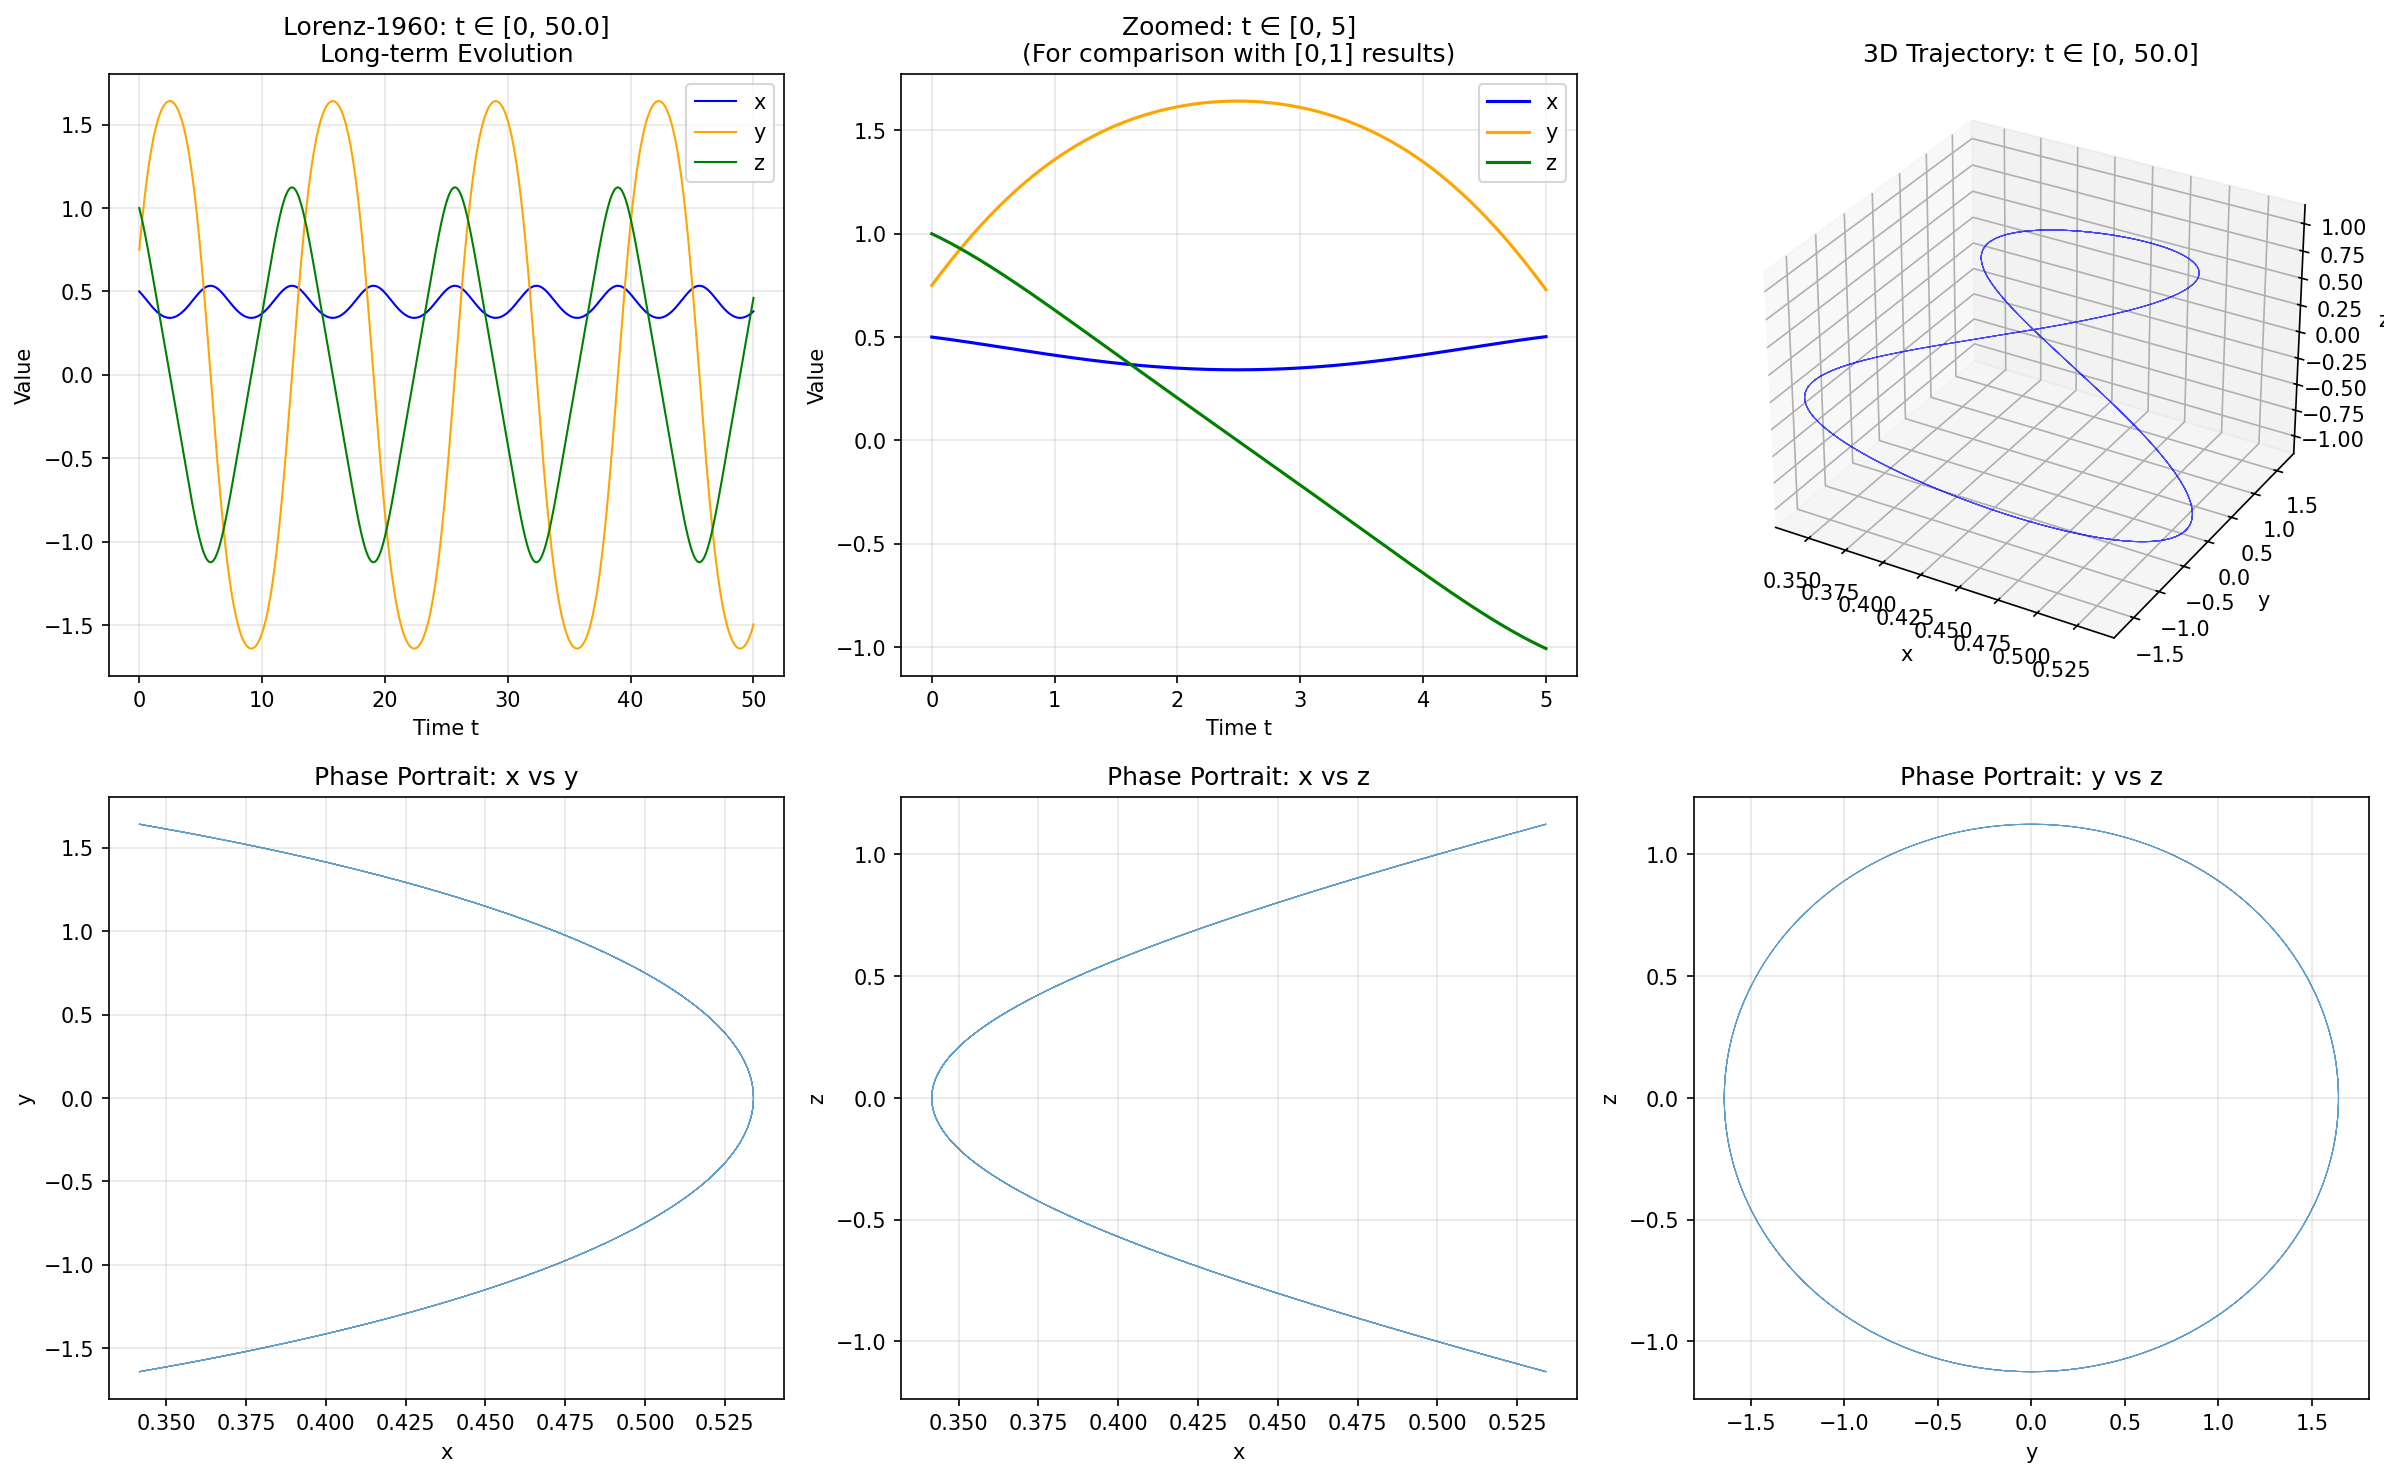
\includegraphics[width=\linewidth]{lorenz1960_extended_time.png}\\
      {\scriptsize Long-term evolution, phase portraits, and 3D trajectory.}
  \end{columns}
\end{frame}

% =============================================================== 6. BACKGROUND: ANN vs PINN
\begin{frame}{Background: Plain ANN vs.\ Physics-Informed NN}
  \begin{columns}[T]
    \column{0.5\textwidth}
      \centering
      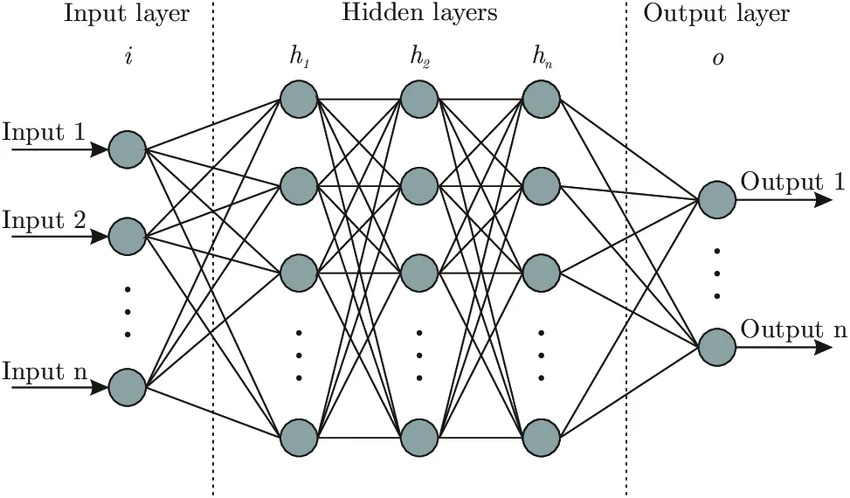
\includegraphics[height=3.0cm]{ann_architecture.jpg}\\[2pt]
      {\footnotesize\textbf{Plain ANN} --- data-driven, learns $t\!\mapsto\!(x,y,z)$ by backpropagation.}
    \column{0.5\textwidth}
      \centering
      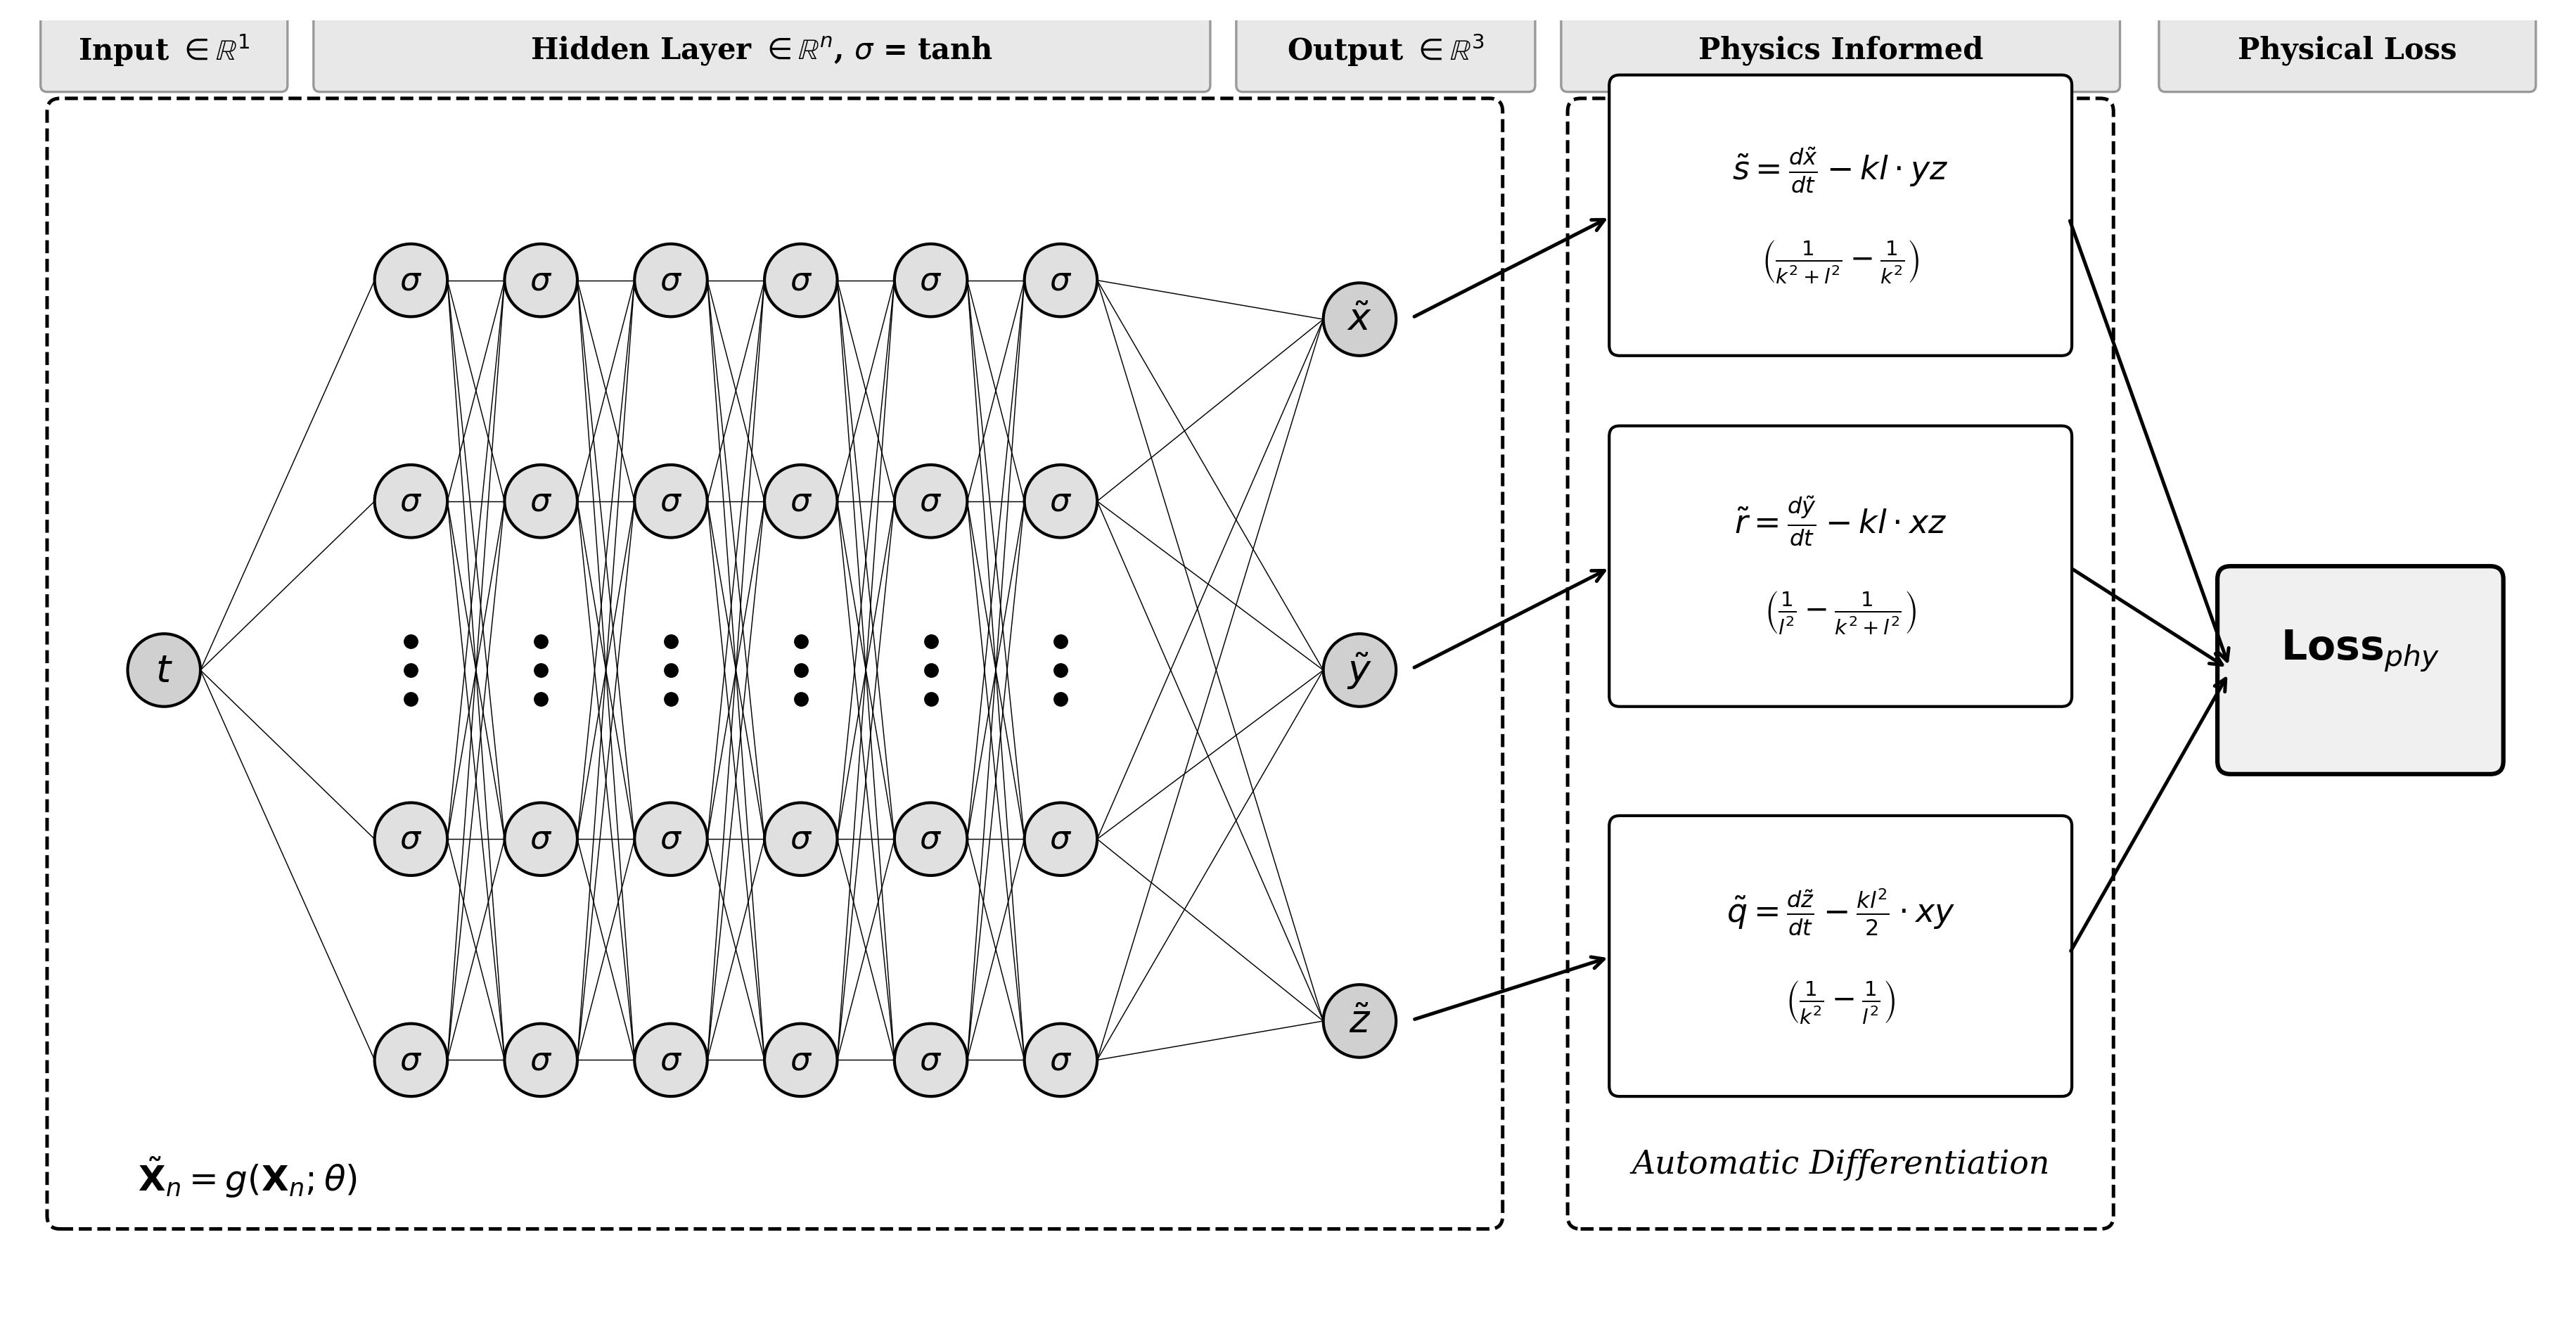
\includegraphics[height=3.0cm]{pinn_architecture.jpg}\\[2pt]
      {\footnotesize\textbf{PINN} --- embeds the governing equations in the loss.}
  \end{columns}
  \vspace{0.3cm}
  \begin{plaincard}
    \centering\footnotesize \textbf{Our scope:} the plain ANN on the left only. PINNs are used as a
    \emph{literature benchmark}, not implemented here.
  \end{plaincard}
\end{frame}

% =============================================================== 7. LITERATURE
\begin{frame}{Literature Review}
  \centering\footnotesize
  \renewcommand{\arraystretch}{1.25}
  \begin{tabular}{>{\raggedright\arraybackslash}p{3.0cm} >{\raggedright\arraybackslash}p{4.0cm} >{\raggedright\arraybackslash}p{4.6cm}}
    \rowcolor{tealDark}
    \textbf{\color{white}Work} & \textbf{\color{white}Approach} & \textbf{\color{white}Gap for our study}\\
    \rowcolor{tealSoft}
    Matthews \& Bihlo (PinnDE) & PINN + DeepONet on Lorenz-1960 & Fixed architecture; physics-informed loss\\
    Aslam et al. & ANN + PSO on a Lorenz variant & Optimises weights, not architecture\\
    \rowcolor{tealSoft}
    Mall \& Chakraverty & ANN, 4--6 nodes, sigmoid only & Simple ODEs; no depth/activation sweep\\
    Lau \& Werth (ODEN) & Plain ANN; tanh/sigmoid $>$ ReLU & No systematic depth--width study\\
    \rowcolor{tealSoft}
    Dubey / Audu et al. & Plain ANN on first-order ODEs & Fixed nets; not coupled, not Lorenz\\
    \textbf{Our work} & \textbf{Plain ANN, systematic search} & \textbf{Depth $\times$ width $\times$ activation on Lorenz-1960}\\
  \end{tabular}
  \vspace{0.25cm}
  \begin{plaincard}
    \centering\scriptsize 17 papers reviewed across PINNs, pure-ANN solvers, architecture studies, Neural ODEs, and hybrids.
  \end{plaincard}
\end{frame}

% =============================================================== 8. GAP + RQ
\begin{frame}{Research Gap \& Questions}
  \begin{columns}[t]
    \column{0.5\textwidth}
      \begin{card}{The gap}
        \footnotesize
        \begin{itemize}
          \item No architecture study for Lorenz-1960
          \item No PINN vs.\ plain-ANN comparison on it
          \item No systematic activation-function study
          \item Depth \emph{and} width rarely varied together
        \end{itemize}
      \end{card}
    \column{0.5\textwidth}
      \begin{card}{Research questions}
        \footnotesize
        \begin{itemize}
          \item Can a plain ANN approximate the Lorenz-1960 solution from numerical data alone?
          \item Which \textbf{depth $\times$ width $\times$ activation} gives the best accuracy--cost trade-off?
          \item How close does it get to physics-informed baselines?
        \end{itemize}
      \end{card}
  \end{columns}
\end{frame}

% =============================================================== 9. METHODOLOGY
\begin{frame}{Methodology: A Two-Phase Comparative Study}
  \begin{columns}[c]
    \column{0.46\textwidth}
      \begin{card}{Phase 1 --- Architecture search}
        \scriptsize
        Depth $\{1,2,3,4\}$ $\times$ width $\{20,50,100\}$ $\times$
        activation $\{$tanh, ReLU, sigmoid, GELU, Swish$\}$\\[3pt]
        \centering{\color{tealDark}\textbf{= 60 runs}} (optimizer fixed: Adam)
      \end{card}
      \vspace{0.15cm}
      \begin{card}{Phase 2 --- Optimizers}
        \scriptsize
        3 best architectures $\times$ \{Adam, L-BFGS, SGD+momentum\}\\[3pt]
        \centering{\color{tealDark}\textbf{= 9 runs}}
      \end{card}
      \vspace{0.15cm}
      \centering{\footnotesize Total: \textbf{69 controlled experiments}}
    \column{0.54\textwidth}
      \centering
      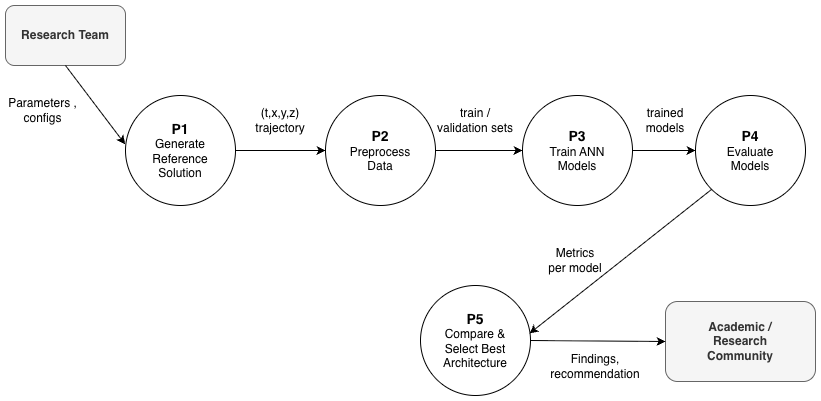
\includegraphics[width=\linewidth]{dfd_level1.png}\\
      {\scriptsize Pipeline: generate $\to$ preprocess $\to$ train $\to$ evaluate $\to$ select.}
  \end{columns}
\end{frame}

% =============================================================== 10. PROGRESS / RESULTS
\begin{frame}{Progress: Validated Numerical Baseline}
  \begin{columns}[c]
    \column{0.58\textwidth}
      \centering
      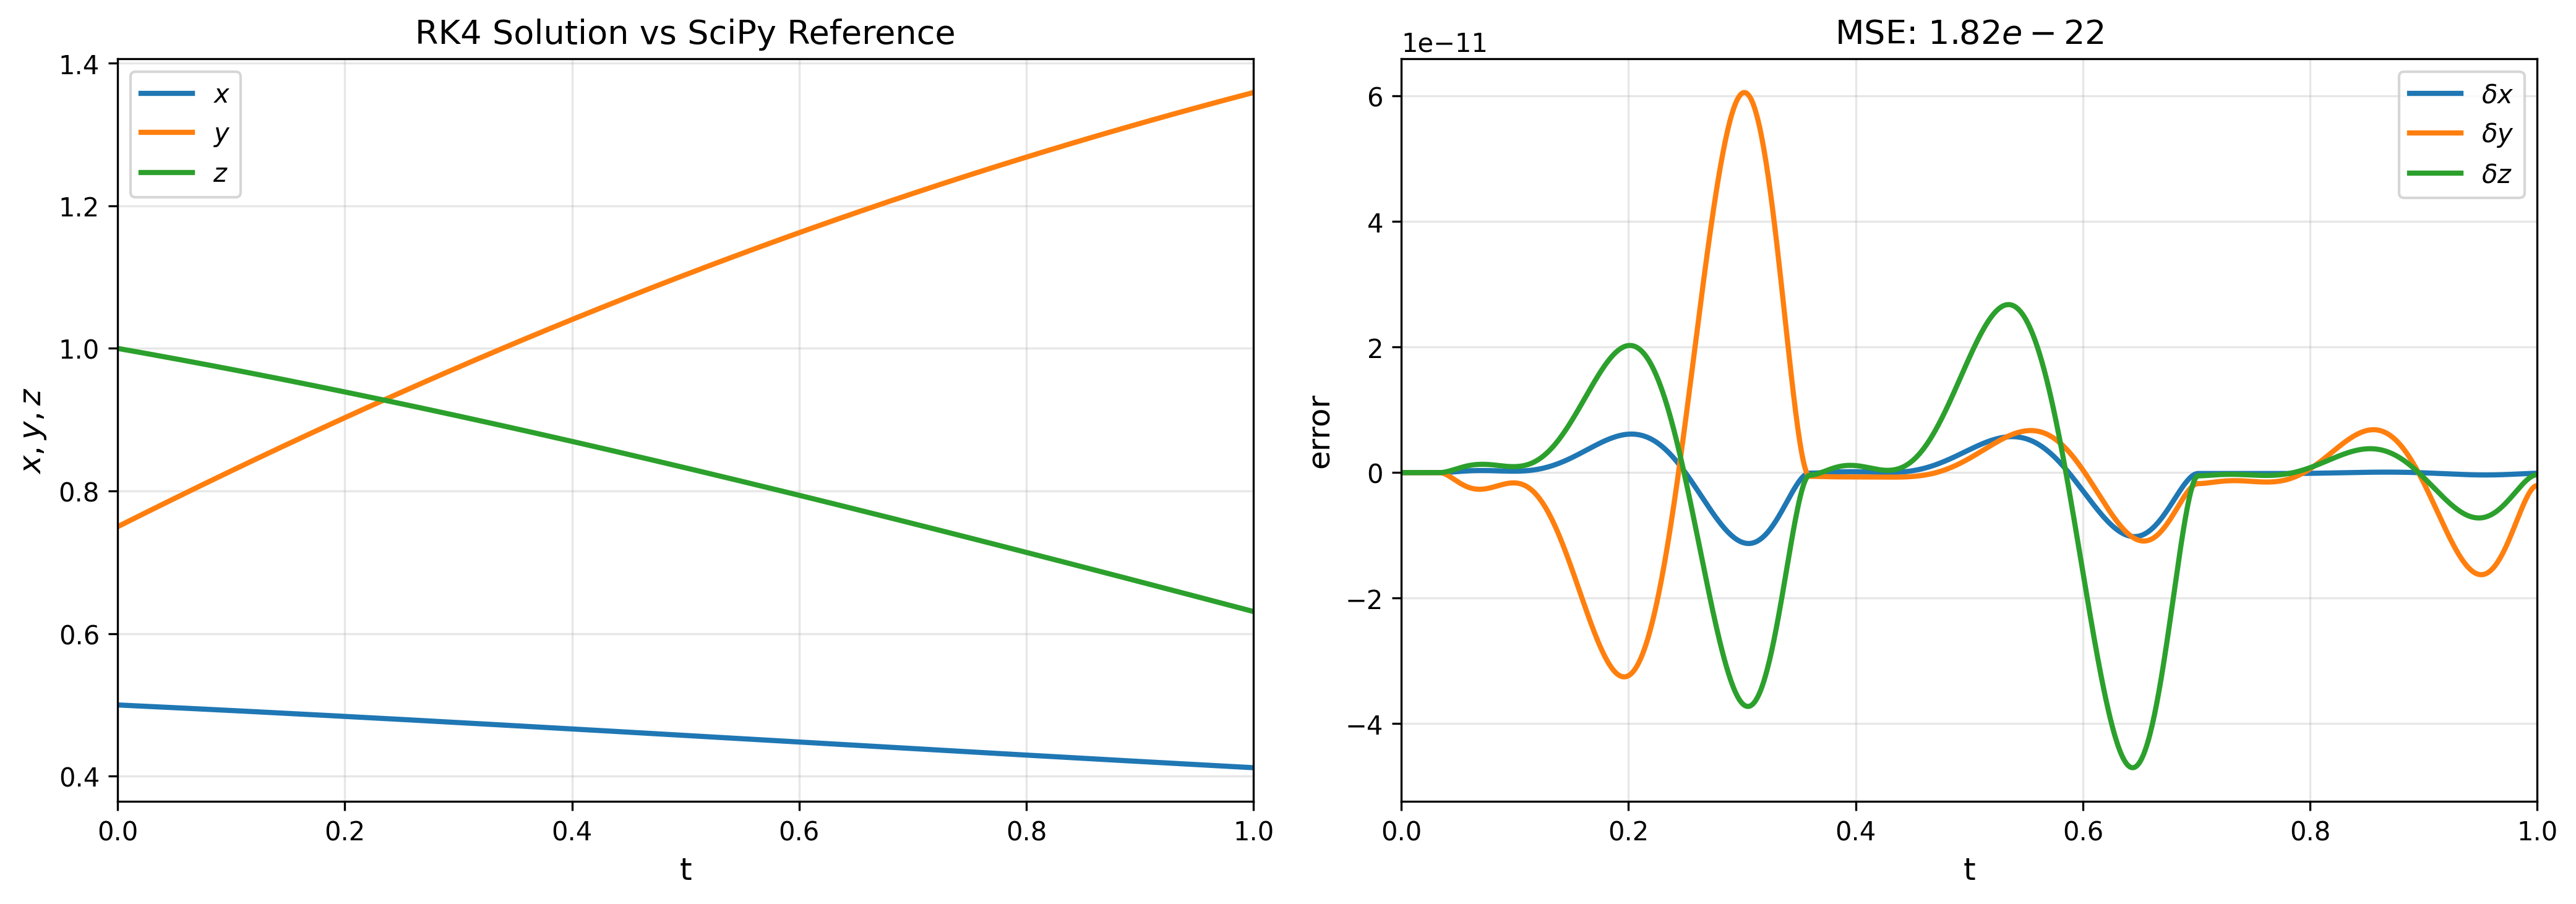
\includegraphics[width=\linewidth]{lorenz1960_comparison.png}\\
      {\scriptsize RK4 vs.\ SciPy DOP853 solution (left) and pointwise error (right).}
    \column{0.42\textwidth}
      \begin{card}{What is done}
        \footnotesize
        \begin{itemize}
          \item Custom RK4 ($h=10^{-3}$, 1001 points)
          \item SciPy DOP853 ($\text{rtol}=10^{-10}$)
          \item Solvers agree to \textbf{MSE $\approx 1.8\times10^{-22}$}
        \end{itemize}
      \end{card}
      \vspace{0.2cm}
      \begin{plaincard}
        \centering\footnotesize The reference trajectory is now a \textbf{defensible ground truth}
        for all ANN training in FYDP-II.
      \end{plaincard}
  \end{columns}
\end{frame}

% =============================================================== 11. PLAN / TIMELINE
\begin{frame}{Project Plan \& FYDP-II Roadmap}
  \footnotesize
  \renewcommand{\arraystretch}{1.2}
  \begin{tabular}{>{\raggedright\arraybackslash}p{2.2cm} >{\raggedright\arraybackslash}p{7.4cm} c}
    \rowcolor{tealDark}
    \textbf{\color{white}Phase} & \textbf{\color{white}Focus} & \textbf{\color{white}Status}\\
    \rowcolor{tealSoft}
    FYDP-I (wk 1--14) & Problem, literature, requirements, \textbf{validated baseline} & {\color{tealDark}\textbf{Done}}\\
    FYDP-II (wk 15--28) & Training pipeline, Phase 1 + Phase 2 runs, metrics \& plots & Next\\
    \rowcolor{tealSoft}
    FYDP-III (wk 29--42) & Reproducibility, comparative analysis, final report \& defense & Planned\\
  \end{tabular}
  \vspace{0.3cm}
  \begin{columns}[t]
    \column{0.5\textwidth}
      \begin{card}{Immediate next steps}
        \scriptsize
        \begin{itemize}
          \item Build the ANN training/eval pipeline
          \item Run the 60 Phase-1 architectures
          \item Select the 3 best for Phase-2
        \end{itemize}
      \end{card}
    \column{0.5\textwidth}
      \begin{card}{Later extensions}
        \scriptsize
        \begin{itemize}
          \item Repeated seeds for stability
          \item Denser grids / new initial conditions
          \item Direct comparison with PINN baselines
        \end{itemize}
      \end{card}
  \end{columns}
\end{frame}

% =============================================================== 12. CONCLUSION
\begin{frame}{Conclusion}
  \begin{columns}[t]
    \column{0.5\textwidth}
      \begin{card}{Where we are}
        \footnotesize
        \begin{itemize}
          \item Clear, narrow research question
          \item 17-paper review with an explicit gap
          \item Two-phase design (69 runs) locked
          \item Dual-solver baseline verified
        \end{itemize}
      \end{card}
    \column{0.5\textwidth}
      \begin{card}{Why it matters}
        \footnotesize
        \begin{itemize}
          \item First systematic plain-ANN architecture study on Lorenz-1960
          \item Clean attribution of architecture vs.\ optimizer effects
          \item Honest scope: claims wait for FYDP-II evidence
        \end{itemize}
      \end{card}
  \end{columns}
  \vspace{0.25cm}
  \begin{plaincard}
    \centering Foundation set --- FYDP-II turns the validated baseline and design into measured results.
  \end{plaincard}
\end{frame}

% =============================================================== 13. REFERENCES
\begin{frame}{Selected References}
  \footnotesize
  \begin{enumerate}
    \item Lorenz, E.N. (1960). Maximum simplification of the dynamic equations. \textit{Tellus}, 12(3).
    \item Matthews, J. \& Bihlo, A. (2024). PinnDE: physics-informed neural networks for ODEs and PDEs.
    \item Raissi, M. et al. (2019). Physics-informed neural networks. \textit{J.\ Comput.\ Phys.}, 378.
    \item Lagaris, I.E. et al. (1998). ANN for solving ODEs and PDEs. \textit{IEEE Trans.\ Neural Netw.}, 9(5).
    \item Lau, K. \& Werth, D. (2020). ODEN: a framework to solve ODEs with neural networks.
    \item Mall, S. \& Chakraverty, S. (2013). Comparison of ANN architectures for ODEs.
    \item Dubey, A. et al. (2024). Solving coupled ODEs using artificial neural networks.
    \item Chen, R.T.Q. et al. (2018). Neural ordinary differential equations. \textit{NeurIPS}.
  \end{enumerate}
  \vspace{0.1cm}
  {\scriptsize Full bibliography (17 works) in the project report, \texttt{paper/final/fydp.bib}.}
\end{frame}

% =============================================================== 14. THANK YOU
{\setbeamertemplate{footline}{}
\begin{frame}[plain]
  \centering
  \vspace{1.1cm}
  {\color{tealDark}\rule{0.7\textwidth}{1.0pt}}\\[0.4cm]
  {\Huge\bfseries Thank you}\\[0.3cm]
  {\Large Questions \& discussion}\\[0.5cm]
  {\color{tealDark}\rule{0.7\textwidth}{1.0pt}}\\[0.6cm]
  {\footnotesize Team Lorenz-1960 $\times$ ANN \textbullet\ Department of CSE, United International University}\\[2pt]
  {\footnotesize Supervisor: Dr.\ Muhammad Nomani Kabir}
\end{frame}
}

\end{document}
